
\newcommand{\param}[2]{\textit{#1}\,--\,#2\,--\,}
\newcommand{\paramnott}[2]{#1\,--\,#2\,--\,}

\chapter{Praktická část}
Praktická část práce se skládá z dvou častí. První část je implementace samotného protokolu L2RS a druhá část je ukázková aplikace která využívá implementaci protokolu. Sekce níže popisují jednotlivé části práce.


\section{Protokol L2RS}
Protokol L2RS je implementovaný v jazyku Python a jako jedinou knihovnu využívá \texttt{numpy}. Parametre pro protokol bili zvolené následovně
\begin{itemize}
  \item \param{q}{12289}modulus pre koeficienty v polynomech,
  \item \param{n}{512}počet koeficientů v polynomech,
  \item \param{m}{6}počet polynomů vo vektoru polynomů,
  \item \paramnott{$\sigma$}{283754}standardní guassova odchylka,
  \item \paramnott{$\gamma$}{13.6}hustota privátního klíče.
\end{itemize}
Tyto parametre bily zvolené aby splňovali bezpečnostní úroveň \texttt{III} protokolu. Vytváření podpisu trvá průměrně 43\,ms a ověření průměrně 38\,ms při výše opomenutých parametrech. Rychlost podpisu a ověření je samozřejmé závislá na parametrech stroje na kterém byli testované. Tyto časy byli měřené na procesoru AMD Ryzen 3600 z frekvencí jádra 3.6\,GHz.

V tabulce \ref{sizes} je možné vidět velkosti jednolitých konstrukcí jako veřejný nebo privátní klíč. Velkosti podpisu jsou lineárně závislé na počtu uživatelů který se zúčastňují podpisu. Velkost podpisu se dá jednoduše vypočítat podle rovnice
\begin{equation}
  S=1792+w*m*896
\end{equation}
kde $w$ označuje počet uživatelů a $m$ je počet polynomech ve jedním vektoru polynomu.

\begin{table}[htbp]
  \centering
  \caption{Velkosti konstrukcí podpisu}
  \begin{tabular}{|l|c|c|}
    \hline
    Typ              & Počet uživatelů & Velkost (B) \\
    \hline
    Veřejný klíč     & -               & 896         \\
    Privátní klíč    & -               & 4480        \\
    Veřejný parametr & -               & 8960        \\
    Podpis           & 1               & 7168        \\
    Podpis           & 2               & 12544       \\
    Podpis           & 5               & 28672       \\
    \hline
  \end{tabular}
  \label{sizes}
\end{table}




\section{Ukázková aplikace}
TODO
Součást práce je taktéž ukázková aplikace která vyváří komunikaci mezi jednolitými uživateli.

\begin{figure}[htbp]
  \centering
  \includegraphics[width=\textwidth]{img/program_output.png}
  \caption{Příklad pro 3 uživatele}
  \label{program_output}
\end{figure}

\begin{figure}[htbp]
  \centering
  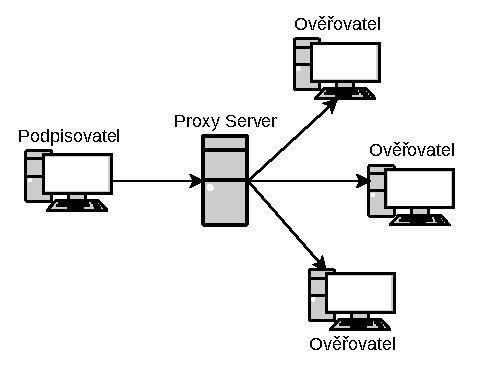
\includegraphics[width=0.7\textwidth]{img/network_diagram.pdf}
  \caption{Sítová komunikace}
  \label{network_diagram}
\end{figure}

\subsection{Návod na použití}
Program používá přepínače na jeho ovládaní. Spuštění je možné ve Windows powershellu, WSL (Windows Subsystem for Linux) a libovolné linux distribuci. Program byl testovaný na verzi \texttt{Python 3.10.7}. Návod na spuštění je následovný. Jako první je potřeba nainstalovat potřebné balíčky pomocí souboru \texttt{requirements.txt} který se nachází v odevzdaném kódu:
\begin{itemize}
  \item \texttt{pip install -r requirements.txt}
\end{itemize}
Spustit \textbf{pouze jeden} proxy server:
\begin{itemize}
  \item \texttt{./ring\_sig.py -sp}
\end{itemize}
Spustit \textbf{pouze jednoho} podpisovatele:
\begin{itemize}
  \item \texttt{./ring\_sig.py -c -s}
\end{itemize}
Spustit \textbf{maximum 255} ověřovatelů:
\begin{itemize}
  \item \texttt{./ring\_sig.py -c -v}
\end{itemize}
Dále stačí jednom zadat text který bude podepsaní a ověřený u každého ověřovatele. Jako předvolené nastavení používá program port \textbf{3000} pro komunikaci. Tento port je možné změnit pomocí přepínače \texttt{-p}.
\begin{itemize}
  \item \texttt{./ring\_sig.py -p [PORT]}
\end{itemize}
Všechny dostupné přepínače se dají zobrazit pomocí:
\begin{itemize}
  \item \texttt{./ring\_sig.py -h}
\end{itemize}
Dále je možné zobrazit jednotlivé parametre které sou použité pro protokol L2RS a sítovou komunikaci:
\begin{itemize}
  \item \texttt{./ring\_sig.py -i}
\end{itemize}


